\documentclass[a4paper]{article}

\usepackage[toc]{appendix}
\usepackage[utf8]{inputenc}
\usepackage[T1]{fontenc}
\usepackage[english]{babel}
\usepackage{geometry}
\usepackage{graphicx}
\usepackage{hyperref}
\usepackage{xcolor}
\usepackage{amsmath}
\usepackage{booktabs}
\usepackage{listings}
\usepackage{fancyhdr}
\usepackage{enumitem}

\geometry{margin=2.5cm}
\hypersetup{
    colorlinks=true,
    linkcolor=black,
    urlcolor=blue,
    citecolor=blue,
    pdftitle={Pepper Robot LLM Chatbot - Technical Report},
    pdfauthor={Balaji S. Bavimane}
}

\definecolor{codegreen}{rgb}{0,0.6,0}
\definecolor{codegray}{rgb}{0.5,0.5,0.5}
\definecolor{codepurple}{rgb}{0.58,0,0.82}
\definecolor{backcolour}{rgb}{0.97,0.97,0.97}
\definecolor{keywordcolor}{rgb}{0.0,0.0,0.7}

\lstdefinestyle{pythonstyle}{
    backgroundcolor=\color{backcolour},
    commentstyle=\color{codegreen},
    keywordstyle=\color{keywordcolor}\bfseries,
    numberstyle=\tiny\color{codegray},
    stringstyle=\color{codepurple},
    basicstyle=\ttfamily\footnotesize,
    breakatwhitespace=false,
    breaklines=true,
    captionpos=b,
    keepspaces=true,
    numbers=left,
    numbersep=5pt,
    showspaces=false,
    showstringspaces=false,
    showtabs=false,
    tabsize=2,
    frame=single,
    framerule=0.5pt
}

\lstdefinestyle{kotlinstyle}{
    backgroundcolor=\color{backcolour},
    commentstyle=\color{codegreen},
    keywordstyle=\color{keywordcolor}\bfseries,
    numberstyle=\tiny\color{codegray},
    stringstyle=\color{codepurple},
    basicstyle=\ttfamily\footnotesize,
    breakatwhitespace=false,
    breaklines=true,
    captionpos=b,
    keepspaces=true,
    numbers=left,
    numbersep=5pt,
    showspaces=false,
    showstringspaces=false,
    showtabs=false,
    tabsize=2,
    frame=single,
    framerule=0.5pt,
    morecomment=[l]{//},
    morekeywords={fun, enum, val, var, class, object, interface, override, suspend, companion, private, public, when, is, sealed, data, lateinit}
}

\lstset{style=pythonstyle}

% Header and footer
\pagestyle{fancy}
\fancyhead[L]{\small Pepper Robot LLM Chatbot}
\fancyhead[R]{\small Development of Robot Applications}
\fancyfoot[C]{\thepage}
\renewcommand{\headrulewidth}{0.4pt}
\renewcommand{\footrulewidth}{0.4pt}

\begin{document}

\begin{titlepage}
    \centering
    \begin{figure}[t]
        \centering
\includegraphics[width=0.3\textwidth]{images/logo.png}
    \end{figure}
    \textsc{\LARGE\bfseries{University of Cagliari \\}}
	  \textsc{\LARGE\bfseries{Faculty of Science\\ }}
    
    \vspace{2cm}
    \LARGE{Development of Robot Applications\\}
    {\Large Project Report}
    \rule{\textwidth}{1pt}\\[0.5cm]
    {\Huge\bfseries Pepper Robot LLM Chatbot}\\[0.3cm]
    {\Large\itshape A Conversational AI System for SoftBank Pepper Robot}\\
    \rule{\textwidth}{1pt}

    \vspace{1cm}
    {\Large\bfseries Submitted by\\}
    \begin{tabular}{rl}
        \Large\textbf{Name:} & \Large Balaji Shivakumarappa Bavimane\\
        \Large\textbf{Matricola:} & \Large IA/66050\\
        \Large\textbf{Date:} & \Large December 30, 2025\\
    \end{tabular}
    
    \vspace{1cm}
    {\Large\bfseries Supervised by\\}
    \Large Prof. Diego Reforgiato Recupero\\Lorenzo Boi
    
    \vfill
    
    \rule{0.6\textwidth}{0.4pt}\\[0.5cm]
    {\small GitHub Repository: \url{https://github.com/balaji1810/Pepper-Robot-Application}\footnote{Installation and setup instructions are available in the project README at the repository link.}}
    \vspace{1cm}
\end{titlepage}

\section*{Abstract}
\addcontentsline{toc}{section}{Abstract}

This report presents the design and implementation of a conversational AI chatbot for the SoftBank Robotics Pepper humanoid robot. The system enables hands-free voice interaction by integrating Android speech recognition with a LangChain-powered Flask backend utilizing the Mistral large language model. Users speak naturally to Pepper, and the robot responds with contextually appropriate answers through its built-in text-to-speech capabilities. The architecture follows a client-server model where the Android application running on Pepper handles speech capture and synthesis, while the Python backend manages conversational context and LLM inference. This project demonstrates practical integration of modern AI capabilities with social robotics, achieving low-latency conversational interaction suitable for educational and assistive applications. The modular design allows for easy extension and adaptation to different use cases.

\newpage
\tableofcontents
\newpage

\section{Introduction}

Human-robot interaction (HRI) has evolved significantly with the advent of large language models (LLMs), enabling more natural and contextually aware conversations between humans and robots. The SoftBank Robotics Pepper robot, designed specifically for social interaction, provides an ideal platform for exploring conversational AI applications. However, integrating modern LLM capabilities with Pepper's existing software ecosystem presents several technical challenges.

This project was undertaken as part of ``Development of Robot Applications'' course. The primary motivation was to explore the practical integration of LangChain-orchestrated LLM inference with Pepper's native speech capabilities, creating a system where users can engage in natural, hands-free conversations with the robot.

\subsection{Motivation}

The inbuilt chatbot implementations on Pepper relied on rule-based dialogue systems services with limited contextual understanding plus its very old and not maintained anymore by SoftBank. The emergence of accessible LLM APIs, combined with orchestration frameworks like LangChain, opens opportunities for more sophisticated conversational capabilities. This project investigates how these technologies can be practically deployed in a robotics context.

\subsection{Scope and Constraints}

The project scope includes:
\begin{itemize}[noitemsep]
    \item Development of a continuous speech recognition system for Pepper
    \item Implementation of a REST API backend with LangChain and Mistral LLM
    \item Session-based conversation memory for contextual responses
    \item Integration with Pepper's QiSDK for text-to-speech synthesis
\end{itemize}

Out of scope for this initial implementation:
\begin{itemize}[noitemsep]
    \item Multi-modal interaction (gestures, facial expressions)
    \item On-device LLM inference
    \item Multi-language support beyond English
    \item Advanced safety filtering mechanisms
\end{itemize}

\section{Objectives}
The project objectives were defined to balance educational learning goals with practical implementation outcomes:

\begin{enumerate}[noitemsep]
    \item \textbf{Understand Pepper SDK Integration:} Gain practical experience with the QiSDK for Android, including robot lifecycle management and speech synthesis.
    
    \item \textbf{Implement Continuous Speech Recognition:} Develop a hands-free automatic speech recognition system that operates continuously without manual intervention.
    
    \item \textbf{Design RESTful API Architecture:} Create a clean, modular Flask API that separates concerns between authentication, request handling, and LLM orchestration.
    
    \item \textbf{Integrate LangChain with Mistral:} Implement conversational AI using LangChain's prompt templates and memory management with the Mistral LLM backend.
    
    \item \textbf{Manage Conversational Context:} Develop session-based memory storage (in-memory and Redis options) to maintain conversation history across interactions.
\end{enumerate}

\section{System Overview}

The Pepper Chatbot system follows a distributed client-server architecture where the Android application on Pepper handles user interaction while the Python backend manages AI inference. This separation allows computational intensive LLM processing to occur on more capable hardware while the robot focuses on real-time speech capture and synthesis.

\subsection{Information Flow}

The conversation flow proceeds through the following stages:
\begin{enumerate}[noitemsep]
    \item User speaks to Pepper's microphone
    \item \texttt{HandsFreeAsr} component transcribes speech to text using Android's SpeechRecognizer
    \item \texttt{ChatApiClient} sends the transcribed text via HTTP POST to the Flask API
    \item Flask API routes the request to the \texttt{ChatAgent} (LangChain chain)
    \item \texttt{ChatAgent} retrieves conversation history, constructs the prompt, and invokes Mistral LLM
    \item LLM response is returned through the API as JSON
    \item \texttt{ChatBotManager} receives the response and uses QiSDK's \texttt{Say} action for speech synthesis
    \item Pepper speaks the response; listening automatically resumes
\end{enumerate}

\subsection{System Architecture Diagram}

Figure~\ref{fig:architecture} illustrates the complete system architecture, showing the interaction between Pepper robot components and the API server.

\begin{figure}[htbp]
    \centering
    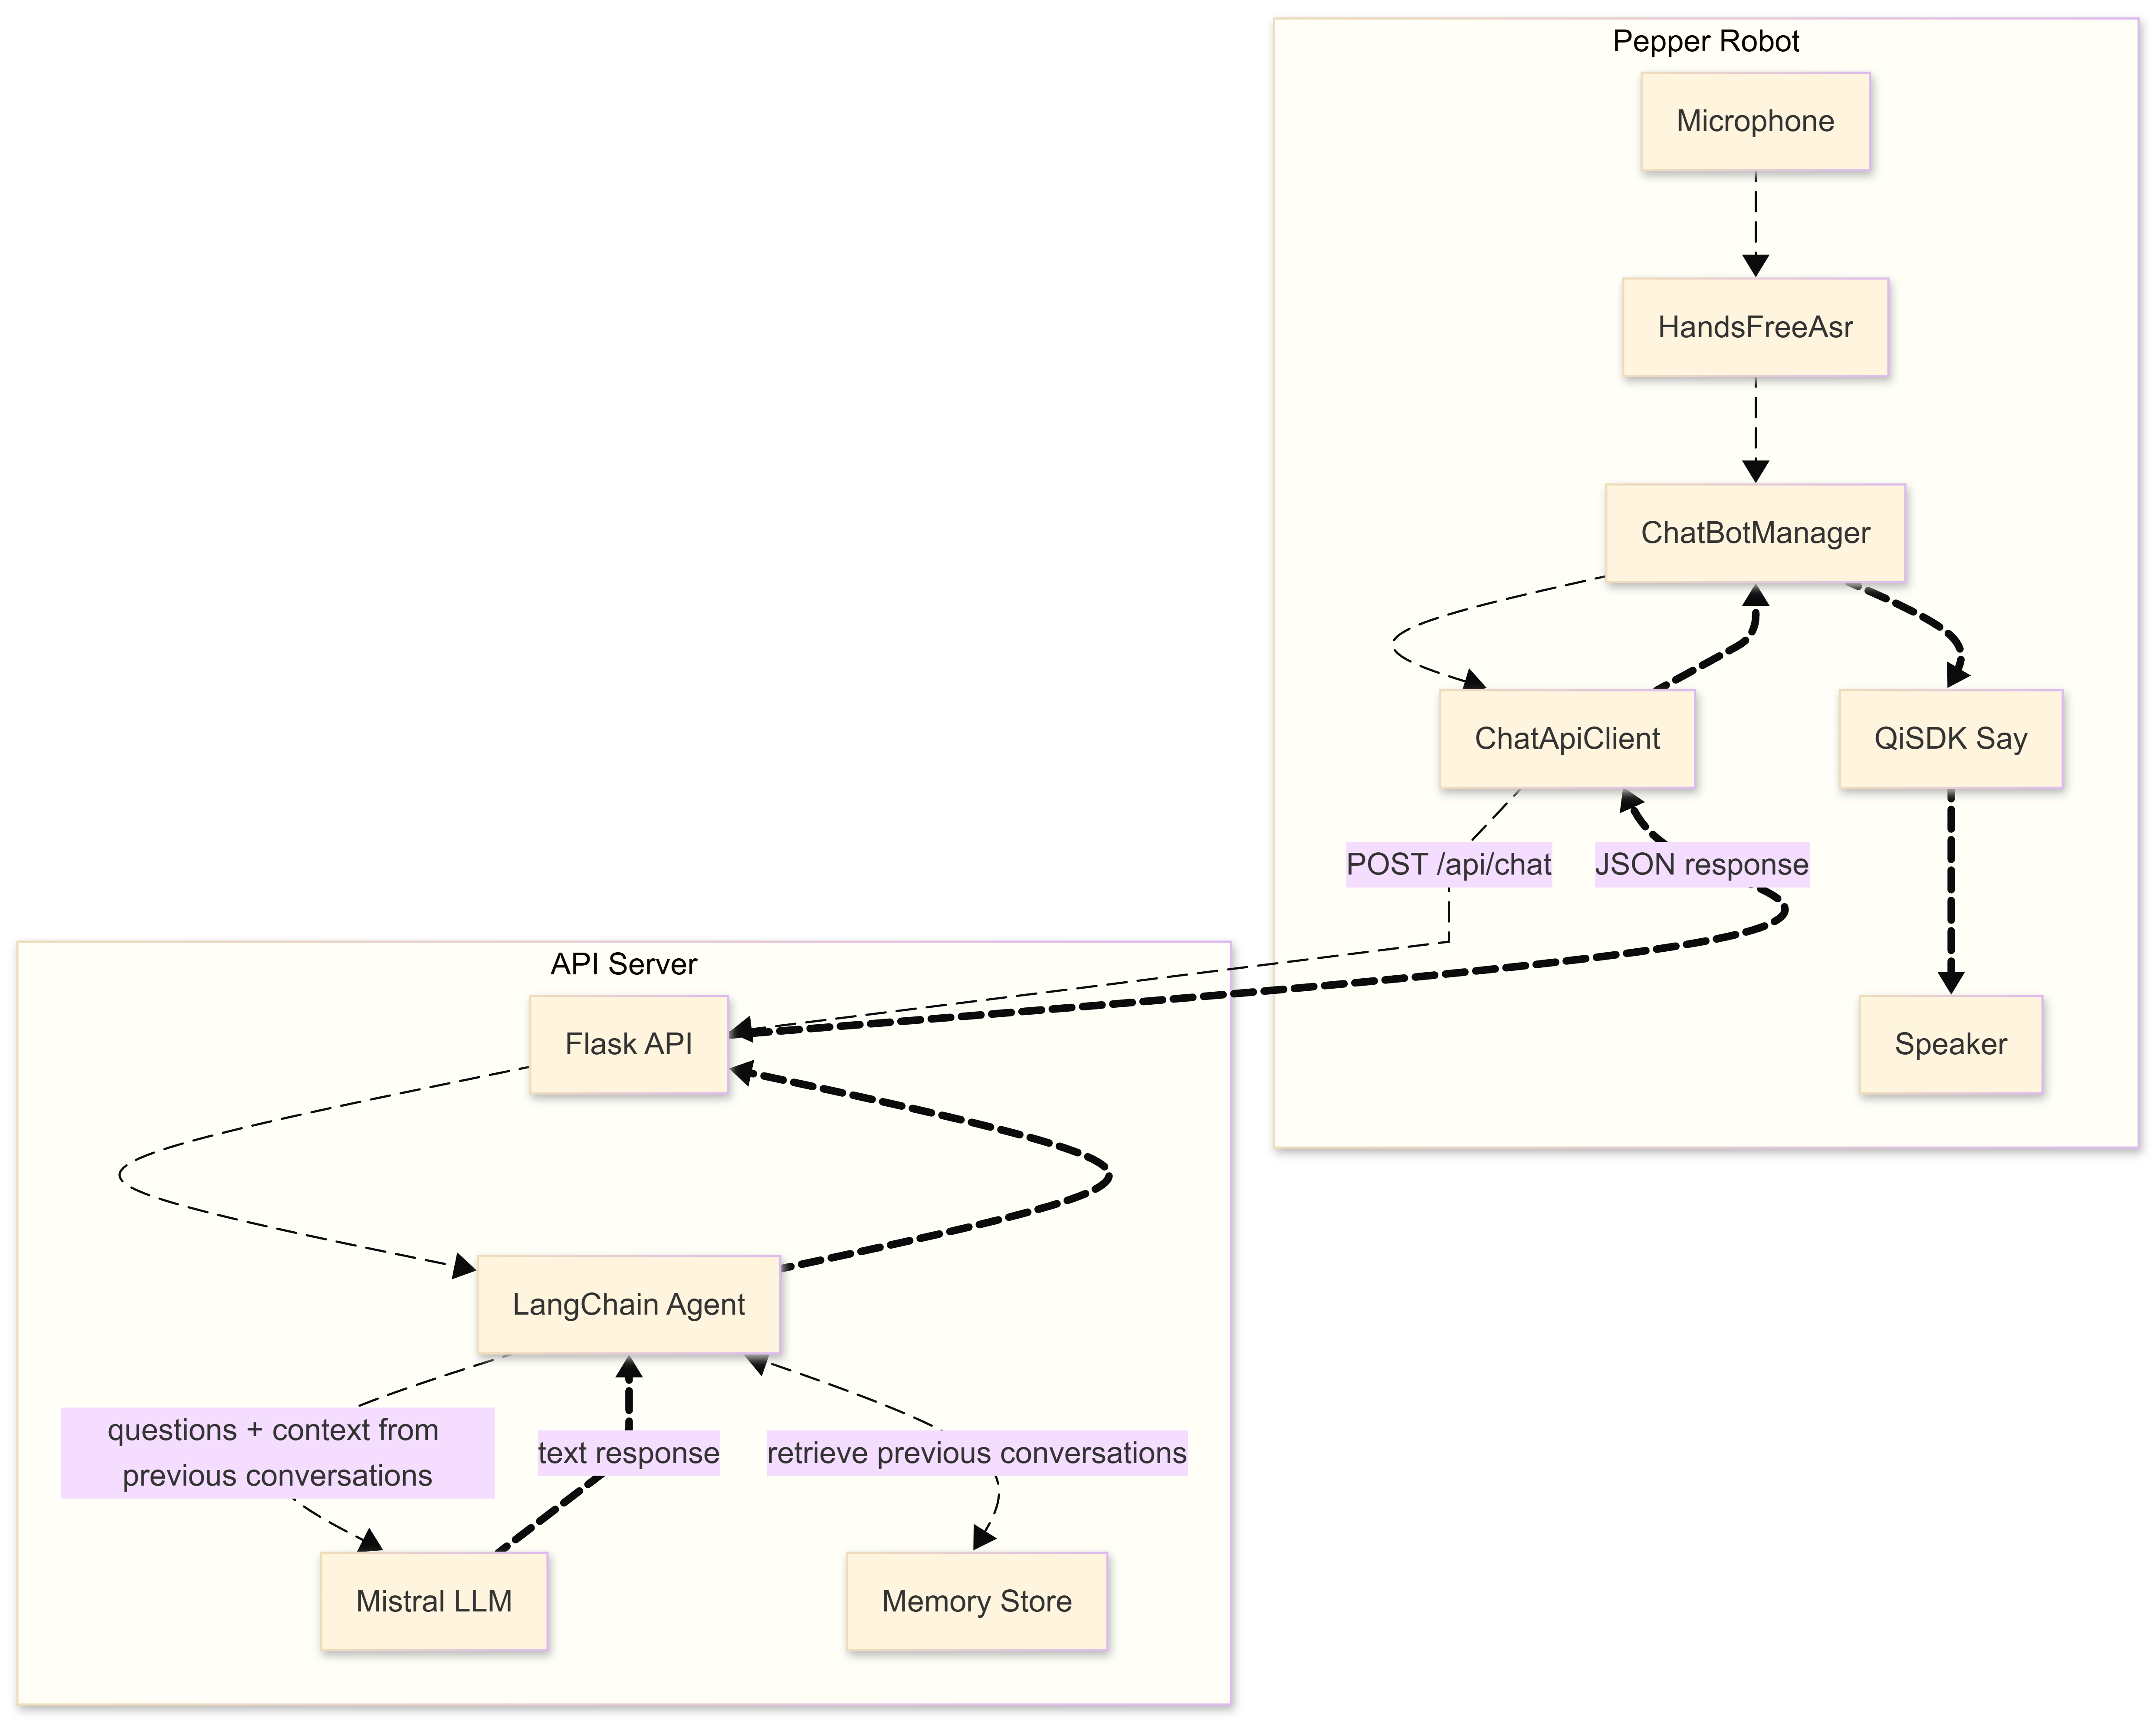
\includegraphics[width=0.95\linewidth]{images/Mermaid Chart - System Architecture.png}
    \caption{System architecture showing the data flow between Pepper Robot components (right) and the API Server (left).}
    \label{fig:architecture}
\end{figure}

\subsection{Component Summary}

Table~\ref{tab:components} summarizes the main system components and their responsibilities.

\begin{table}[htbp]
    \centering
    \caption{System Component Overview}
    \label{tab:components}
    \begin{tabular}{@{}lp{9cm}@{}}
        \toprule
        \textbf{Component} & \textbf{Description} \\
        \midrule
        HandsFreeAsr & Android SpeechRecognizer wrapper providing continuous voice input with automatic restart \\
        ChatBotManager & Orchestrates API calls and Pepper speech synthesis; manages conversation state \\
        ChatApiClient & HTTP client sending JSON messages to the Flask backend \\
        Flask API & REST endpoint wrapping the LangChain agent with Bearer token authentication \\
        ChatAgent & LangChain conversational chain with Mistral LLM and session memory \\
        Memory Store & Session-based storage (in-memory or Redis) for conversation history \\
        QiSDK Say & Pepper's native text-to-speech action for verbal output \\
        \bottomrule
    \end{tabular}
\end{table}

\section{Detailed Design}
\label{sec:detailed-design}

This section provides detailed descriptions of each system component, including design rationale and key implementation aspects.

\subsection{Android Pepper Application}
\label{subsec:android-app}

The Android application is structured around four main classes, following separation of concerns principles.

\subsubsection{MainActivity}

\texttt{MainActivity} serves as the central orchestrator, implementing both \texttt{RobotLifecycleCallbacks} for QiSDK integration and listener interfaces for ASR and ChatBot events. Key responsibilities include:

\begin{itemize}[noitemsep]
    \item Managing Android activity lifecycle and permissions
    \item Coordinating robot focus acquisition/loss
    \item Bridging ASR results to the ChatBot manager
    \item Updating the conversation display UI
\end{itemize}

The activity maintains state flags (\texttt{isActivityVisible}, \texttt{hasRobotFocus}, \texttt{hasAudioPermission}) to ensure listening only occurs when all prerequisites are met.

\subsubsection{HandsFreeAsr}

The \texttt{HandsFreeAsr} class encapsulates all speech recognition logic, providing a clean interface to the activity. Key design decisions include:

\begin{itemize}[noitemsep]
    \item \textbf{Automatic restart:} After each utterance or physiological error (no speech, no match, timeout), listening automatically restarts with a configurable delay.
    \item \textbf{Error categorization:} Errors are classified as ``physiological'' (recoverable) or ``blocking'' (requiring intervention), enabling appropriate handling. See Appendix~\ref{app:asr-error}
\end{itemize}

Listing~\ref{lst:asr-intent} shows the configuration of the speech recognition intent.

\begin{lstlisting}[style=kotlinstyle, caption={Speech recognition intent configuration in HandsFreeAsr}, label=lst:asr-intent]
private fun createRecognizerIntent(): Intent {
    return Intent(RecognizerIntent.ACTION_RECOGNIZE_SPEECH).apply {
        putExtra(RecognizerIntent.EXTRA_LANGUAGE_MODEL, RecognizerIntent.LANGUAGE_MODEL_FREE_FORM)
        putExtra(RecognizerIntent.EXTRA_LANGUAGE, language.toLanguageTag())
        putExtra(RecognizerIntent.EXTRA_PARTIAL_RESULTS, true)
        putExtra(RecognizerIntent.EXTRA_MAX_RESULTS, 3)
        putExtra(RecognizerIntent.EXTRA_SPEECH_INPUT_MINIMUM_LENGTH_MILLIS, 3000L)
        putExtra(RecognizerIntent.EXTRA_SPEECH_INPUT_COMPLETE_SILENCE_LENGTH_MILLIS, 1500L)
    }
}
\end{lstlisting}

\subsubsection{ChatApiClient}

The \texttt{ChatApiClient} handles HTTP communication with the Flask backend using Kotlin coroutines for asynchronous operation. The client:

\begin{itemize}[noitemsep]
    \item Constructs JSON request bodies with user text and session ID
    \item Includes Bearer token authentication headers
    \item Implements 30-second timeout handling
    \item Provides sealed class responses (\texttt{Success} or \texttt{Error}) for type-safe result handling
\end{itemize}

\subsubsection{ChatBotManager}

The \texttt{ChatBotManager} coordinates the conversation flow, managing three states: \texttt{IDLE}, \texttt{PROCESSING}, and \texttt{SPEAKING}. It:

\begin{itemize}[noitemsep]
    \item Prevents overlapping requests when busy
    \item Maintains conversation history for UI display
    \item Invokes QiSDK's \texttt{SayBuilder} for speech synthesis
    \item Requests ASR pause during processing and speaking
\end{itemize}

Listing~\ref{lst:speak-response} shows the speech synthesis implementation.\\
Appendix~\ref{app:states} shows different implementations of the states.
\begin{lstlisting}[style=kotlinstyle, caption={Speech synthesis using QiSDK in ChatBotManager}, label=lst:speak-response]
private fun speakResponse(text: String) {
    val context = qiContext ?: return
    state = State.SPEAKING
    listener.onSpeakingStarted()

    speakingJob = scope.launch {
        withContext(Dispatchers.IO) {
            val say: Say = SayBuilder.with(context)
                .withText(text)
                .withLocale(Locale(Language.ENGLISH, Region.UNITED_STATES))
                .build()
            say.run()
        }
        state = State.IDLE
        listener.onSpeakingFinished()
        listener.onResumeAsrRequested()
    }
}
\end{lstlisting}

\subsection{Flask LangChain API}

The Python backend follows a modular structure with clear separation between configuration, authentication, routing, and AI logic.

\subsubsection{Application Factory Pattern}

The \texttt{main.py} module uses Flask's application factory pattern, creating the app with configured dependencies:

\begin{lstlisting}[language=Python, caption={Flask application factory in main.py}, label=lst:flask-factory]
def create_app() -> Flask:
    config = load_config()
    
    # Choose memory store based on config
    if config.USE_REDIS and config.REDIS_URL:
        memory = RedisStore(config.REDIS_URL)
    else:
        memory = InMemoryStore()

    agent = ChatAgent(config=config, memory_store=memory)
    app = Flask(__name__)
    app.before_request(require_api_token(config))
    app.register_blueprint(create_api(agent))
    
    @app.route("/health")
    def health():
        return {"status": "ok"}

    return app
\end{lstlisting}

\subsubsection{API Endpoint}

The \texttt{/api/chat} endpoint handles POST requests with JSON validation:

\begin{itemize}[noitemsep]
    \item Enforces \texttt{application/json} content type
    \item Validates required \texttt{text} field (max 2000 characters)
    \item Auto-generates session IDs if not provided
    \item Returns structured JSON responses with \texttt{ok}, \texttt{session\_id}, and \texttt{reply} fields
\end{itemize}

\subsubsection{Request/Response Format}

The API uses a simple JSON schema for communication:

\textbf{Request:}
\begin{lstlisting}[language=Python, caption={API request JSON schema}]
{
    "text": "Hello, how are you?",
    "session_id": "user123"  // optional
}
\end{lstlisting}

\textbf{Response:}
\begin{lstlisting}[language=Python, caption={API response JSON schema}]
{
    "ok": true,
    "session_id": "user123",
    "reply": "Hello! I'm doing well, thank you for asking."
}
\end{lstlisting}

\subsubsection{Authentication}
Bearer token authentication is implemented as a Flask \texttt{before\_request} handler, validating the \texttt{Authorization} header against the configured token.

\subsection{LangChain Integration}
\label{subsec:langchain}

The \texttt{ChatAgent} class implements the conversational AI logic using LangChain's composable architecture.

\subsubsection{Prompt Engineering}

The prompt template includes a system prompt establishing the assistant's persona and constraints:

\begin{lstlisting}[language=Python, caption={System prompt and template in chain.py}, label=lst:prompt]
SYSTEM_PROMPT = (
    "You are a helpful assistant for a Pepper robot. "
    "You must respond politely, concisely (<= 200 words), "
    "and avoid giving legal/medical advice."
)

PROMPT_TEMPLATE = (
    "System: " + SYSTEM_PROMPT + "\n\n"
    "Conversation so far:\n{history}\n\n"
    "User: {user_input}\nAssistant:"
)
\end{lstlisting}

\subsubsection{Chain Construction}

The agent uses \href{https://blog.langchain.com/langchain-expression-language/}{LangChain Expression Language (LCEL)} to compose the processing pipeline:

\begin{lstlisting}[language=Python, caption={LangChain chain construction}, label=lst:chain]
self.llm = ChatMistralAI(
    temperature=config.LLM_TEMPERATURE,
    max_retries=2,
    timeout=30,
)
self.prompt = PromptTemplate(
    input_variables=["history", "user_input"],
    template=PROMPT_TEMPLATE,
)
# Simple chain: prompt -> llm -> parser
self.chain = self.prompt | self.llm | StrOutputParser()
\end{lstlisting}
See Appendix~\ref{app:reply} to see how to invoke this chain.

\subsubsection{Conversation Memory}

The memory store maintains session-based conversation history as a list of (user, assistant) tuples. Two implementations are provided:

\begin{itemize}[noitemsep]
    \item \texttt{InMemoryStore}: Dictionary-based storage for development/single-instance deployment
    \item \texttt{RedisStore}: Redis list-based storage with TTL (24 hours) for cloud deployment
\end{itemize}
See Appendix~\ref{app:redis} and Appendix~\ref{app:inmemory} for detailed implementation.

\subsection{Data Flow Diagram}

Table~\ref{tab:dataflow} summarizes the data transformations at each stage.

\begin{table}[htbp]
    \centering
    \caption{Data Flow Summary}
    \label{tab:dataflow}
    \begin{tabular}{@{}llp{6cm}@{}}
        \toprule
        \textbf{Stage} & \textbf{Format} & \textbf{Content} \\
        \midrule
        Speech Input & Audio & Raw audio from Pepper microphone \\
        ASR Output & String & Transcribed text (e.g., ``Hello Pepper'') \\
        API Request & JSON & \texttt{\{text, session\_id\}} \\
        LLM Prompt & String & Formatted prompt with history \\
        LLM Response & String & Generated response text \\
        API Response & JSON & \texttt{\{ok, session\_id, reply\}} \\
        TTS Input & String & Reply text for synthesis \\
        Speech Output & Audio & Pepper's spoken response \\
        \bottomrule
    \end{tabular}
\end{table}

\section{Implementation Notes}

\subsection{Threading and Asynchronous Behavior}

The Android application uses Kotlin coroutines for asynchronous operations:
\begin{itemize}[noitemsep]
    \item \texttt{Dispatchers.IO} for network requests and blocking QiSDK calls
    \item \texttt{Dispatchers.Main} for UI updates
    \item \texttt{SupervisorJob} to prevent coroutine cancellation propagation
\end{itemize}

\subsection{Error Handling Strategy}

The system implements error handling:

\begin{itemize}[noitemsep]
    \item \textbf{Network errors:} Timeout, connection refused, and other network issues return appropriate HTTP status codes (408, 502, 415, 500...)
    \item \textbf{ASR errors:} Classified into recoverable (auto-restart) and blocking (require user action)
    \item \textbf{LLM errors:} Timeout detection via exception message parsing; automatic retries configured in LangChain
\end{itemize}

\subsection{Configuration Management}

Environment-based configuration uses \texttt{python-dotenv} for the backend:

\begin{table}[htbp]
    \centering
    \caption{Configuration Variables}
    \label{tab:config}
    \begin{tabular}{@{}lp{8cm}@{}}
        \toprule
        \textbf{Variable} & \textbf{Description} \\
        \midrule
        MISTRAL\_API\_KEY & API key for Mistral AI (required) \\
        API\_AUTH\_TOKEN & Bearer token for API authentication (required) \\
        FLASK\_HOST & Server bind address (default: 0.0.0.0) \\
        FLASK\_PORT & Server port (default: 5000) \\
        USE\_REDIS & Enable Redis session storage (0 or 1) \\
        REDIS\_URL & Redis connection URL \\
        LLM\_TEMPERATURE & LLM creativity parameter (0.0--1.0) \\
        \bottomrule
    \end{tabular}
\end{table}

\subsection{Security Considerations}

The implementation includes basic security measures:
\begin{itemize}[noitemsep]
    \item Bearer token authentication prevents unauthorized API access
    \item Input length validation (2000 character limit) mitigates prompt injection risks
    \item API keys are loaded from environment variables, not hardcoded
\end{itemize}

\section{Evaluation and Testing}

\subsection{Testing Methodology}

The system was evaluated through manual testing scenarios on a physical Pepper robot connected to a local network. Testing focused on:

\begin{itemize}[noitemsep]
    \item End-to-end conversation flow
    \item Error recovery behavior
    \item Session continuity across multiple exchanges
\end{itemize}

\subsection{Example Dialogues}

Table~\ref{tab:dialogues} presents representative interaction samples demonstrating system behavior.

\begin{table}[htbp]
    \centering
    \caption{Example Conversation Exchanges}
    \label{tab:dialogues}
    \begin{tabular}{@{}p{5cm}p{8cm}@{}}
        \toprule
        \textbf{User Input} & \textbf{Pepper Response} \\
        \midrule
        ``Hi Pepper, how are you?'' & ``Hello! I'm doing well, thank you for asking. How can I assist you today?'' \\
        \midrule
        ``What can you help me with?'' & ``I can help you with various tasks such as answering questions, providing information, or simply having a conversation. What would you like to know?'' \\
        \midrule
        ``Tell me a fun fact about robots.'' & ``Here's a fun fact: The word 'robot' comes from the Czech word 'robota,' meaning forced labor. It was first used in a 1920 play by Karel Čapek.'' \\
        \bottomrule
    \end{tabular}
\end{table}

The system successfully maintained conversation context across multiple turns, with the session ID mechanism enabling continuity.

\section{Limitations and Risks}

\subsection{Technical Limitations}

\begin{itemize}[noitemsep]
    \item \textbf{Network dependency:} Requires stable WiFi connection between Pepper and API server.
    \item \textbf{Single language:} Currently configured for English.
    \item \textbf{No streaming:} Responses are not streamed; full generation must complete before speaking.
    \item \textbf{Memory limitations:} In-memory store loses sessions on server restart.
    \item \textbf{No offline fallback:} System non-functional without API connectivity.
\end{itemize}

\subsection{Known Issues}

\begin{itemize}[noitemsep]
    \item ASR may occasionally produce spurious empty results requiring restart.
    \item Long responses may exceed comfortable listening duration.
    \item No mechanism to interrupt Pepper while speaking.
\end{itemize}

\subsection{Safety and Privacy Concerns}

\begin{itemize}[noitemsep]
    \item \textbf{LLM hallucination:} Model may generate incorrect or inappropriate content.
    \item \textbf{Data transmission:} User speech is sent to external Mistral API servers.
    \item \textbf{No content filtering:} Beyond the system prompt, no explicit safety filters are implemented.
\end{itemize}

\section{Discussion and Lessons Learned}

\subsection{What Worked Well}

\begin{itemize}[noitemsep]
    \item \textbf{Modular architecture:} Clear separation between components facilitated development and debugging
    \item \textbf{LangChain integration:} The framework simplified LLM orchestration and prompt management
    \item \textbf{QiSDK compatibility:} Pepper's SDK integrated with standard Android patterns after some modifications\footnote{The "QiSDK Plugin" for Android Studio was published in 2017, but as of 2025 it is no longer compatible with Android Studio. I used \href{https://github.com/unitedroboticsgroup-france/MyPepperApplication?tab=readme-ov-file\#pepper-with-android-studio-in-2024}{this} guide to use latest version of Android Studio with Pepper, without the need of the plugin.}
    \item \textbf{Conversation history:} Simple tuple-based memory proved effective for maintaining context
\end{itemize}

\subsection{Challenges Encountered}

\begin{itemize}[noitemsep]
    \item \textbf{QiSDK reliability:} The \href{https://qisdk.softbankrobotics.com/sdk/doc/pepper-sdk/index.html}{Pepper SDK for Android} provided by SoftBank robotics is relatively old and not maintained properly for latest versions of android studio.
    \item \textbf{Timing coordination:} Preventing ASR from listening while Pepper speaks required careful state management.
    \item \textbf{Response length control:} LLM may sometimes generates longer responses than ideal for spoken interaction.
\end{itemize}

\subsection{Suggestions for Improvement}

\begin{itemize}[noitemsep]
    \item Implement response streaming to reduce perceived latency
    \item Add configurable wake word detection like ``Ok Pepper'' or ``Hey Pepper'' to automatically start listening
    \item Integrate gesture and expression alongside speech
    \item Deploy safety filters (toxicity detection, topic restrictions)
\end{itemize}

\section{Future Work}

\begin{itemize}
    \item \textbf{Safety and Content Filtering:} Implement moderation API calls or local classifiers to filter inappropriate LLM outputs before speech synthesis.
    \item \textbf{Response Streaming:} Use Server-Sent Events or WebSockets to stream partial responses, enabling Pepper to begin speaking before full generation completes.
    \item \textbf{On-Device Inference:} Explore smaller LLMs (e.g., Phi, Gemma) that could run on a companion device for offline operation.
    \item \textbf{Multi-Modal Interaction:} Integrate Pepper's gesture capabilities to complement verbal responses with appropriate body language.
    \item \textbf{Multi-Language Support:} Extend ASR configuration to support multiple languages with automatic detection.
    \item \textbf{User Personalization:} Store user preferences and adapt responses based on interaction history.
\end{itemize}

\section{Conclusions}

This project successfully demonstrated the integration of modern large language model capabilities with the SoftBank Pepper robot platform. The resulting system enables natural, hands-free conversational interaction where users speak to Pepper and receive contextually appropriate verbal responses.

Key achievements include:
\begin{itemize}[noitemsep]
    \item A functional end-to-end conversational system from speech input to robot speech output
    \item Clean, modular architecture separating Android client and Python backend concerns
    \item Session-based conversation memory enabling multi-turn dialogue
    \item Comprehensive error handling for reliable operation
\end{itemize}

The project provided valuable learning experiences in robot application development, Android SDK integration, REST API design, and LLM orchestration with LangChain. While limitations exist, particularly regarding safety filtering and offline operation, the system provides a solid foundation for future enhancements and demonstrates the feasibility of deploying LLM-powered conversational AI on social robots.

\bibliographystyle{plain}
\addcontentsline{toc}{section}{References}
\nocite{*}
\bibliography{main}
\newpage

\begin{appendices}

\section{Libraries and Versions}

\subsection{Python Backend:}
\begin{itemize}[noitemsep]
    \item flask 3.1.2
    \item python-dotenv 1.2.1
    \item redis 7.1.0
    \item langchain 1.2.0
    \item langchain-mistralai 1.1.1
\end{itemize}

\subsection{Android Application:}
\begin{itemize}[noitemsep]
    \item Kotlin 2.0.21
    \item Android Gradle Plugin 8.13
    \item QiSDK 1.7.5
    \item AndroidX Core KTX 1.10.1
    \item AndroidX Compose BOM 2024.09.00
    \item AndroidX Activity Compose 1.8.0
\end{itemize}

\section{Selected Code Excerpts}
\label{app:code}

\subsection{ASR Error Handling}
\label{app:asr-error}
Error categorization for appropriate recovery behavior:

\begin{lstlisting}[style=kotlinstyle, caption={ASR error handling from HandsFreeAsr.kt}]
sealed class AsrError(val message: String) {
    // Physiological errors - can automatically restart
    class NoSpeech : AsrError("No speech detected")
    class NoMatch : AsrError("Speech not recognized")
    class Timeout : AsrError("Speech timeout")

    // Blocking errors - require user intervention
    class PermissionDenied : AsrError("Microphone permission denied")
    class AudioError : AsrError("Audio recording error")
    class NetworkError : AsrError("Network error")
    class NotAvailable : AsrError("Speech recognition not available")

    val isPhysiological: Boolean
        get() = this is NoSpeech || this is NoMatch || this is Timeout
}
\end{lstlisting}

\subsection{States of the application}
\label{app:states}
Different states of \texttt{ChatBotManager}. When $state \neq IDLE$ any new message from the user will be ignored.
\begin{lstlisting}[style=kotlinstyle, caption={enum State from ChatBotManager.kt}, label=lst:chatbot-states]
enum class State {
    IDLE,           // Waiting for user input
    PROCESSING,     // Sending to API and waiting for response
    SPEAKING        // Pepper is speaking the response
}
\end{lstlisting}

Different states of speech recognizer. When $state = PROCESSING$ speech recognition will be paused temporarily.
\begin{lstlisting}[style=kotlinstyle, caption={enum State from HandsFreeAsr.kt}, label=lst:asr-states]
// Represents the internal state of the ASR.
enum class State {
    IDLE,           // Not listening, microphone inactive
    LISTENING,      // Microphone active, waiting for speech
    SPEECH_ACTIVE,  // User is currently speaking
    PROCESSING      // Processing the utterance (after speech ends)
}
\end{lstlisting}

Each state in the \texttt{ChatState} enum represents a phase in the conversation flow:
\begin{itemize}[noitemsep]
    \item \texttt{INITIALIZING} – App is starting up and setting up components
    \item \texttt{IDLE} – System is ready but not actively listening or processing
    \item \texttt{LISTENING} – ASR is active and waiting for the user to speak
    \item \texttt{USER\_SPEAKING} – User has started speaking and voice is being captured
    \item \texttt{PROCESSING} – User's speech has ended; sending to API and awaiting response
    \item \texttt{BOT\_SPEAKING} – Pepper robot is speaking the bot's response aloud
    \item \texttt{ERROR} – Something went wrong (permission denied, ASR unavailable, API error, etc.)
\end{itemize}
\begin{lstlisting}[style=kotlinstyle, caption={enum ChatState from MainActivity.kt}, label=lst:ui-states]
// Represents the overall chat state for UI updates.
enum class ChatState {
    INITIALIZING,
    IDLE,
    LISTENING,
    USER_SPEAKING,
    PROCESSING,
    BOT_SPEAKING,
    ERROR
}
\end{lstlisting}

\subsection{ChatAgent Reply Method}
\label{app:reply}
The core method that processes user messages and generates responses:

\begin{lstlisting}[language=Python, caption={ChatAgent.reply() method from chain.py}]
def reply(self, session_id: str, text: str) -> str:
    history_pairs = self.memory_store.get(session_id)
    history_str = format_history(history_pairs)

    try:
        response: str = self.chain.invoke({
            "history": history_str,
            "user_input": text,
        })
    except Exception as e:
        msg = str(e).lower()
        if "timeout" in msg or "timed out" in msg:
            raise TimeoutError("LLM timeout")
        raise

    # Update memory
    try:
        self.memory_store.append(session_id, text, response)
    except Exception:
        logger.exception("Failed to append to memory store")

    return response
\end{lstlisting}

\subsection{RedisStore Implementation}
\label{app:redis}
Cloud session storage using Redis lists:

\begin{lstlisting}[language=Python, caption={RedisStore class from memory\_store.py}]
ConversationPair = tuple[str, str]

class RedisStore():
    def __init__(self, redis_url: str, ttl_seconds: int = 86400) -> None:
        self._client = redis.Redis.from_url(redis_url, decode_responses=True)
        self._ttl = ttl_seconds
        self._sep = "\u241E"  # Separator for user/assistant text

    def _key(self, session_id: str) -> str:
        return f"pepper:chat:{session_id}"

    def get(self, session_id: str) -> list[ConversationPair]:
        key = self._key(session_id)
        items = self._client.lrange(key, 0, -1)
        result = []
        for raw in items:
            user, assistant = raw.split(self._sep, 1)
            result.append((user, assistant))
        if result:
            self._client.expire(key, self._ttl)  # Extend TTL
        return result

    def append(self, session_id: str, user_text: str, 
               assistant_text: str) -> None:
        key = self._key(session_id)
        payload = f"{user_text}{self._sep}{assistant_text}"
        pipeline = self._client.pipeline()
        pipeline.rpush(key, payload)
        pipeline.expire(key, self._ttl)
        pipeline.execute()
\end{lstlisting}

\subsection{InMemoryStore Implementation}
\label{app:inmemory}
In memory session storage using python's list and tuple
\begin{lstlisting}[language=Python, caption={InMemoryStore class from memory\_store.py}]

class InMemoryStore():

    def __init__(self) -> None:
        self._store: dict[str, list[ConversationPair]] = {}

    def get(self, session_id: str) -> list[ConversationPair]:
        return list(self._store.get(session_id, []))

    def append(self, session_id: str, user_text: str, assistant_text: str) -> None:
        self._store.setdefault(session_id, []).append((user_text, assistant_text))
\end{lstlisting}

\section{Installation Note}
\label{app:install}

Complete installation and setup instructions, including Python environment configuration, Android Studio setup, and Pepper robot deployment procedures, are available in the project README at:

\begin{center}
    \url{https://github.com/balaji1810/Pepper-Robot-Application}
\end{center}

\end{appendices}

\end{document}
